\documentclass{math}

\usepackage{float}
\usepackage{graphicx}
\usepackage{subcaption}

\geometry{letterpaper, margin=0.5in}

\title{Intro to Computer Vision: HW 3}
\author{Alvin Lin}
\date{August 2018 - December 2018}

\begin{document}

\maketitle
\captionsetup{justification=centering}

\subsection*{Part A}
I implemented the \texttt{load\_images()} function by using regular expressions
to parse the filename for the azimuth and elevation and the \texttt{os} module
to fetch all the files in the data directories. As a result, the
\texttt{num\_images} parameter ended up unused. \par
I implemented the pseudocode for photometric stereo as described in the
assignment using many of the operations provided by \texttt{numpy}. The fast
vector manipulations made many of the transpositions and calculations
very easy. From the height map, you can see horizontal lines across the face as
differences in shade. This is likely due to variations in illumination across
the entire image dataset which become exaggerated by the integration process.
The scale of height is also not properly captured by this process, since peaks
such as the regions around the nose and the chin are not proportioned correctly.

\subsection*{Part B}
\begin{figure}[H]
  \begin{subfigure}{0.35\linewidth}
    \centering
    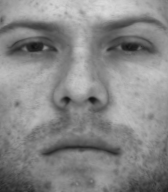
\includegraphics[width=4cm]{assets/hw_03_albedo.png}
    \caption{Albedo image for yaleB01}
  \end{subfigure}
  \begin{subfigure}{0.3\linewidth}
    \centering
    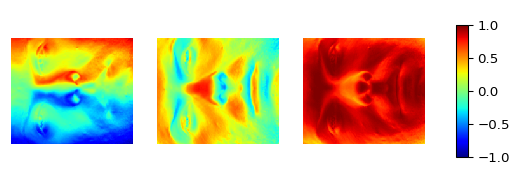
\includegraphics[width=12cm]{assets/hw_03_surface_normals.png}
    \caption{Surface normals for yaleB01}
  \end{subfigure}
\end{figure}
\begin{figure}[H]
  \begin{subfigure}{0.33\linewidth}
    \centering
    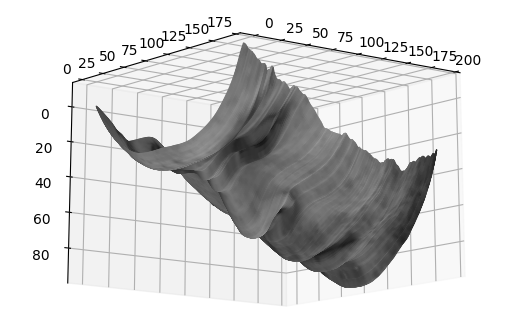
\includegraphics[width=5cm]{assets/hw_03_height_map_01.png}
  \end{subfigure}
  \begin{subfigure}{0.33\linewidth}
    \centering
    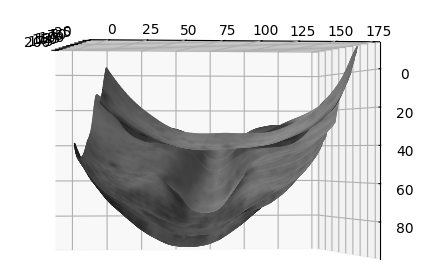
\includegraphics[width=5cm]{assets/hw_03_height_map_02.png}
  \end{subfigure}
  \begin{subfigure}{0.33\linewidth}
    \centering
    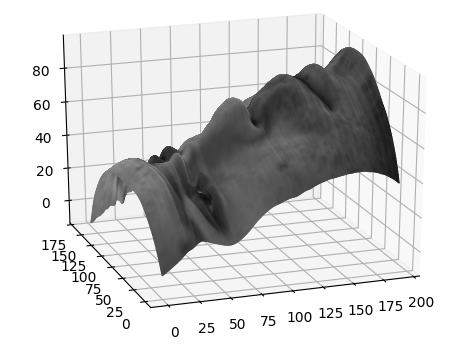
\includegraphics[width=5cm]{assets/hw_03_height_map_03.png}
  \end{subfigure}
  \caption{Height map of yaleB01}
\end{figure}

\subsection*{Part C}
Many of the assumptions about illumination with regard to shape from shading are
not true due to the nature of the surface. With shape from shading, we assume
that the surface does not reflect light, but in reality, light bounces off of
regions around our face (especially our nose) and contributes to the lighting of
nearby features. The eye in particular tends to reflect a lot of light, which is
evident from the fact that the area around the eyelid and eyeball are not
correctly proportioned in our height map reconstruction. The eye position and
the hair in all the images is also not uniform across the dataset, which can
contribute to some error as seen in the examples below.
\begin{figure}[H]
  \begin{subfigure}{0.5\linewidth}
    \centering
    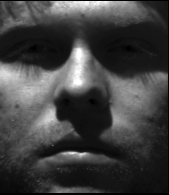
\includegraphics[width=5cm]{assets/hw_03_yaleB01_01.png}
    \caption{Hair shadows are visible in this image}
  \end{subfigure}
  \begin{subfigure}{0.5\linewidth}
    \centering
    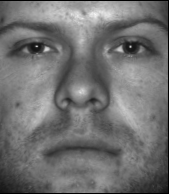
\includegraphics[width=5cm]{assets/hw_03_yaleB01_02.png}
    \caption{Light is reflected off the person's forehead}
  \end{subfigure}
\end{figure}

\begin{center}
  If you have any questions, comments, or concerns, please contact me at
  alvin@omgimanerd.tech
\end{center}

\end{document}
